%!TeX program = xelatex
\documentclass[10pt]{beamer}

\usetheme{metropolis}
\usepackage{appendixnumberbeamer}
\usepackage{booktabs}
\usepackage[scale=2]{ccicons}
\usepackage{pgfplots}
\usepackage{color}
\usepgfplotslibrary{dateplot}
\usepackage{xspace}
\newcommand{\themename}{\textbf{\textsc{metropolis}}\xspace}

\usepackage{stmaryrd}
\usepackage{amsmath}
\usepackage{verbatim}
\usepackage{tikz}
\usepackage{siunitx}
\usepackage{color}
\usepackage[normalem]{ulem}
\usetikzlibrary{calc,decorations.pathmorphing,patterns}
\usepackage{amssymb}
\usepackage{amsfonts}
\usepackage{amscd}
\usepackage{amsthm}
\usepackage{mathrsfs}
\usepackage{enumerate}
\usepackage{mathtools}
\usepackage{booktabs}
\usepackage{array}
\usepackage{nth}
\usepackage{lipsum}
\usetikzlibrary{decorations.markings}


%%%%%%%%%%%%%%%%%%%%%%%%%%%%%list %%%%%%%%%%%%%%%%%
\usepackage{textcomp}           % To use with matlab-prettifier
\usepackage{listings}
\usepackage[framed , numbered]{matlab-prettifier}
\usepackage{listings}
%%%%%%%%%%%%%%%%%end of list%%%%%%%%%%%%%%%%%%%%%

%%%%%%%%%%%%%%%%%%%%%%%%%%%%%%%%%%%%%%%%%%%%%%%%%%%%%%%%%%%%%%%%%%%%%%%%%
%%%% The following is for fancy box %%%%%%%%%%%%%%
\usepackage[framemethod=TikZ]{mdframed}
%%%%%%%%%%%%% Theorem %%%%%%%%%%%%
\newenvironment{thm}[2][]{%
\ifstrempty{#1}%
{\mdfsetup{%
frametitle={%
\tikz[baseline=(current bounding box.east),outer sep=0pt]
\node[anchor=east,rectangle,fill=red!20]
{\strut Theorem};}}
}%
{\mdfsetup{%
frametitle={%
\tikz[baseline=(current bounding box.east),outer sep=0pt]
\node[anchor=east,rectangle,fill=red!20]
{\strut Theorem #1};}}%
}%
\mdfsetup{innertopmargin=1pt,linecolor=red!20,%
linewidth=2pt,topline=true,%
frametitleaboveskip=\dimexpr-\ht\strutbox\relax
}
\begin{mdframed}[]\relax%
\label{#2}}{\end{mdframed}}
%%%%%%%%%%%%%%Lemma%%%%%%%%%%%%%%%%%%%%%%%%%%%%%%%%%%%%%%%%%%%%%%%%%%%%%%
\newcounter{lem}[section] \setcounter{lem}{0}
\renewcommand{\thelem}{}
\newenvironment{lem}[2][]{%
\refstepcounter{lem}%
\ifstrempty{#1}%
{\mdfsetup{%
frametitle={%
\tikz[baseline=(current bounding box.east),outer sep=0pt]
\node[anchor=east,rectangle,fill=green!20]
{\strut Lemma~\thelem};}}
}%
{\mdfsetup{%
frametitle={%
\tikz[baseline=(current bounding box.east),outer sep=0pt]
\node[anchor=east,rectangle,fill=green!20]
{\strut Lemma~\thelem:~#1};}}%
}%
\mdfsetup{innertopmargin=1pt,linecolor=green!20,%
linewidth=2pt,topline=true,%
frametitleaboveskip=\dimexpr-\ht\strutbox\relax
}
\begin{mdframed}[]\relax%
\label{#2}}{\end{mdframed}}
%%%%%%%%%%%%%%%%%%%%%%%%%%%%%%%%%%%%%%%%%%%%%%%%%%%%%%%%%%%%%%%%%%%%%%%
%Corollary
\newenvironment{cor}[2][]{%
\ifstrempty{#1}%
{\mdfsetup{%
frametitle={%
\tikz[baseline=(current bounding box.east),outer sep=0pt]
\node[anchor=east,rectangle,fill=blue!30]
{\strut Corollary};}}
}%
{\mdfsetup{%
frametitle={%
\tikz[baseline=(current bounding box.east),outer sep=0pt]
\node[anchor=east,rectangle,fill=blue!30]
{\strut Corollary:~#1};}}%
}%
\mdfsetup{innertopmargin=1pt,linecolor=blue!30,%
linewidth=2pt,topline=true,%
frametitleaboveskip=\dimexpr-\ht\strutbox\relax
}
\begin{mdframed}[]\relax%
\label{#2}}{\end{mdframed}}
%%%%%%%%%%%%%%%%%%%%%%%%%%%%%%%%%%%%%%%%%%%%%%%%%%%%%%%%%%%%%%%%%%%%%%%
%Proof
\newenvironment{prove}[2][]{%
\ifstrempty{#1}%
{\mdfsetup{%
frametitle={%
\tikz[baseline=(current bounding box.east),outer sep=0pt]
\node[anchor=east,rectangle,fill=red!20]
{\strut Proof};}}
}%
{\mdfsetup{%
frametitle={%
\tikz[baseline=(current bounding box.east),outer sep=0pt]
\node[anchor=east,rectangle,fill=red!20]
{\strut Proof:~#1};}}%
}%
\mdfsetup{innertopmargin=1pt,linecolor=red!20,%
linewidth=2pt,topline=true,%
frametitleaboveskip=\dimexpr-\ht\strutbox\relax
}
\begin{mdframed}[]\relax%
\label{#2}}{\end{mdframed}}
%%%%%%%%%%%%%%%%%%%%%%%%%%%%%%%%%%%%%%%%%%%%%%%%%%%%%%%%%%%%%%%%%%%%%%%
%Defintion
\newcounter{drf}[section]\setcounter{drf}{0}
\renewcommand{\thedrf}{}
\newenvironment{drf}[2][]{%
\refstepcounter{drf}%
\ifstrempty{#1}%
{\mdfsetup{%
frametitle={%
\tikz[baseline=(current bounding box.east),outer sep=0pt]
\node[anchor=east,rectangle,fill=orange!20]
{\strut Definition~\thedrf};}}
}%
{\mdfsetup{%
frametitle={%
\tikz[baseline=(current bounding box.east),outer sep=0pt]
\node[anchor=east,rectangle,fill=orange!20]
{\strut Definition~\thedrf:~#1};}}%
}%
\mdfsetup{innertopmargin=1pt,linecolor=orange!20,%
linewidth=2pt,topline=true,%
frametitleaboveskip=\dimexpr-\ht\strutbox\relax
}
\begin{mdframed}[]\relax%
\label{#2}}{\end{mdframed}}
%%%%%%%%%%%%%%%%%%%%%%%%%%%%%%%%%%%%%%%%%%%%%%%%%%%%%%%%%%%%%%%%%%%%%%%%%%%
% end of self defined label
%%%%%%%%%%%%%%%%%%%%%%%%%%%%%%%%%%%%%%%%%%%%%%%%%%%%%%%%%%%%%%%%%%%%%%%%%%%


%%%%%%%%%%%%%% For double curly bracket%%%%%%%%%%%%%%%%
\usepackage{xparse}

\NewDocumentCommand{\dgal}{sO{}m}{%
  \IfBooleanTF{#1}
    {\dgalext{#3}}
    {\dgalx[#2]{#3}}%
}

\NewDocumentCommand{\dgalext}{m}{%
  \sbox0{%
    \mathsurround=0pt % just for safety
    $\left\{\vphantom{#1}\right.\kern-\nulldelimiterspace$%
  }%
  \sbox2{\{}%
  \ifdim\ht0=\ht2
    \{\kern-.45\wd2 \{#1\}\kern-.45\wd2 \}%
  \else
    \left\{\kern-.5\wd0\left\{#1\right\}\kern-.5\wd0\right\}%
  \fi
}

\NewDocumentCommand{\dgalx}{om}{%
  \sbox0{\mathsurround=0pt$#1\{$}%
  \sbox2{\{}%
  \ifdim\ht0=\ht2
    \{\kern-.45\wd2 \{#2\}\kern-.45\wd2 \}%
  \else
    \mathopen{#1\{\kern-.5\wd0 #1\{}
    #2
    \mathclose{#1\}\kern-.5\wd0 #1\}}
  \fi
}
%%%%%%%%%%%%%%%%



%%%%%%%%%%%%%%%%%%%%%%%%%%%%%%%%%%%%%

\usepackage{animate}

\graphicspath{{./fig/}}


%%%%%%%%%%%%%% define color %%%%%%%%%%%%%%%%%%
\definecolor{DarkFern}{HTML}{407428}
\definecolor{DarkCharcoal}{HTML}{4D4944}
\colorlet{Fern}{DarkFern!85!white}
\colorlet{Charcoal}{DarkCharcoal!85!white}
\colorlet{LightCharcoal}{Charcoal!50!white}
\colorlet{AlertColor}{orange!80!black}
\colorlet{DarkRed}{red!70!black}
\colorlet{DarkBlue}{blue!70!black}
\colorlet{DarkGreen}{green!70!black}

\newcommand{\I}{\mathrm{i}}




%%%%%%%%%%%%%%%%%%%%%%%%%%%%%%%%%%%%%%
%\newcommand{\G}{\alert{G}}  % change color of main author



%%%%%%%%%%%%% Title Page %%%%%%%%%%%%%%%%%%%

\title{MAST90026 Computational Differential\\Equations: Week 8}
%\subtitle{A modern beamer theme}
\date{Semester 1 2024}
\author{Jesse Collis\\Modified from Hailong Guo (2022)}
\institute{The University of Melbourne}
\titlegraphic{\vspace{6cm}\flushright\includegraphics[height=2cm]{logo.png}}


\begin{document}

\maketitle


%
%
%\begin{frame}{Table of contents}
%  \setbeamertemplate{section in toc}[sections numbered]
%  \tableofcontents[hideallsubsections]
%\end{frame}


%-=-=-=-=-=-=-=-=-=-=-=-=-=-=-=-=-=-=-=-=-=-=-=-=
%
%	SECTION: 
%
%-=-=-=-=-=-=-=-=-=-=-=-=-=-=-=-=-=-=-=-=-=-=-=-=
%\section{Method of Weighted Residuals}








%-=-=-=-=-=-=-=-=-=-=-=-=-=-=-=-=-=-=-=-=-=-=-=-=
%	FRAME:
%-=-=-=-=-=-=-=-=-=-=-=-=-=-=-=-=-=-=-=-=-=-=-=-=
\begin{frame}{Evolution PDEs}
\alert{Classical examples}:
\begin{align*}
  & u_t = u_{xx}, \quad \quad \quad \quad \quad \text{diffusion equation},\\
  & u_t + cu_x = 0, \quad \quad \quad  \text{transport equation},\\
  &u_{tt} = c^2 u_{xx}, \quad \quad \quad \quad  \text{wave equation},
\end{align*}


Focus on \mbox{1+1 D} (i.e. time + $x$) problems and \mbox{1+2D} (i.e. time +$x,y$. \mbox{1+3} D problems can be solved using the same techniques just trickier implementation.

\vspace{0.5em}
We can think of \mbox{1+1 D} PDEs as adding time to a BVP or adding space to an IVP.
To be well posed, typically we will need both boundary conditions (like a BVP) and initial conditions (like an IVP).



\end{frame}
   



%-=-=-=-=-=-=-=-=-=-=-=-=-=-=-=-=-=-=-=-=-=-=-=-=
%	FRAME:
%-=-=-=-=-=-=-=-=-=-=-=-=-=-=-=-=-=-=-=-=-=-=-=-=
\begin{frame}{Parabolic equation}

Consider
\begin{equation*}
u_t - (D(x)u')' + q(x)u=r(x),
\end{equation*}
 with
\begin{align*}
\mbox{BCs}: u(a,t)= \alpha(t),\\
u(b,t)=\beta(t),\\
\mbox{IC}: u(x,0)=u_0(x).
\end{align*}
If $D=1$, $q=0$, $r=0$ then this is the heat/diffusion equation.
 
 
 \vspace{0.5em}
 Two classes of numerical methods:
 \begin{itemize}
 	\item Semi-discretisation 
 	\item Full discrete
 \end{itemize}
 
\end{frame}



%-=-=-=-=-=-=-=-=-=-=-=-=-=-=-=-=-=-=-=-=-=-=-=-=
%	FRAME:
%-=-=-=-=-=-=-=-=-=-=-=-=-=-=-=-=-=-=-=-=-=-=-=-=
\begin{frame}{Semi-discretisation (Method of line)}

Idea: discretise in space only, e.g.\ FD, FEM, finite volume, spectral,  collocation .etc. as before. This produces  a system of ODEs that we solve with an 
IVP package e.g. $ode45$ in {\textbf{Matlab}}. 

\vspace{0.5em}

For larger problems, we need to discretise in time as well, e.g.\ if our IVP solver cannot handle the system of ODEs. This gives \emph{fully discrete methods}.


\vspace{0.5em}

But for modest problems the Method of Lines (MoL) is a good approach. 


\end{frame}




%-=-=-=-=-=-=-=-=-=-=-=-=-=-=-=-=-=-=-=-=-=-=-=-=
%	FRAME:
%-=-=-=-=-=-=-=-=-=-=-=-=-=-=-=-=-=-=-=-=-=-=-=-=
\begin{frame}{Semi-discretisation: Finite difference method for space}

Consider the problem
\[  u_t - (D(x)u_x)_x = r(x,t).\]


\begin{center}
	    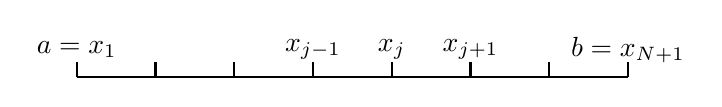
\begin{tikzpicture}
  \draw[color=black, thick] (0,0) -- (1, 0) -- (2, 0) -- (3, 0) -- (4, 0) -- (5, 0) -- (6, 0) -- (7, 0);
  \foreach \x in {0,...,7}
  {
  \draw[color=black, thick] (\x, 0) -- (\x, 0.2);
  }
  \node at (0, 0.35) {$a = x_1$};
    \node at (7, 0.35) {$b = x_{N+1}$};
     \node at (3, 0.35) {$ x_{j-1}$};
      \node at (4, 0.35) {$ x_{j}$};
       \node at (5, 0.35) {$x_{j+1}$};

\end{tikzpicture}
\end{center}


\vspace{0.5em}


When we have an equation in flux form (or conservative form) e.g. from a conservation law, it's good practice to discretize each derivative separately, 
rather than expand derivatives and then discretize, i.e.  $(D(x) u_x)_x$ rather than $D'(x) u_x + D(x) u_{xx}$. 
\end{frame}





%-=-=-=-=-=-=-=-=-=-=-=-=-=-=-=-=-=-=-=-=-=-=-=-=
%	FRAME:
%-=-=-=-=-=-=-=-=-=-=-=-=-=-=-=-=-=-=-=-=-=-=-=-=
\begin{frame}{Semi-discretisation: Finite difference scheme}

Discretise $-(D(x)u_x)_x$ using central differences. We can use FD on
$-D(x)u_x$ directly without expanding it.

\begin{align*}
\left.D(x)u_x\right|_{x_j} &\approx \frac{D(x_j)(u_{j+1/2} - u_{j - 1/2})}{h}, \\
\left.(D(x)u_x)_x\right|_{x_j} &\approx \frac{\left.D(x)u_x\right|_{x_{j+1/2}} - \left.D(x)u_x\right|_{x_{j-1/2}}}{h} \\
&= \frac{1}{h}\left( \frac{D(x_{j+1/2})(u_{j+1} - u_{j})}{h} - \frac{D(x_{j-1/2})(u_{j} - u_{j - 1})}{h}\right) \\
&= \frac{1}{h^2}\left( D(x_{j+1/2})u_{j+1} - (D(x_{j+1/2}) + D(x_{j-1/2}))u_j + D(x_{j-1/2})u_{j-1} \right).
\end{align*}





\end{frame}





%-=-=-=-=-=-=-=-=-=-=-=-=-=-=-=-=-=-=-=-=-=-=-=-=
%	FRAME:
%-=-=-=-=-=-=-=-=-=-=-=-=-=-=-=-=-=-=-=-=-=-=-=-=
\begin{frame}{Semi-discretisation: Dirichlet boundary condition}

Add Dirichlet boundary conditions:
$$ u_1(t) = \alpha(t), \qquad u_{N+1}(t) = \beta(t). $$
Therefore at positions $j=2,\ldots,N$ we have the following equations:
$$ \dot{u}_j(t) - \frac{1}{h^2}\left( D(x_{j+1/2})u_{j+1} - (D(x_{j+1/2}) + D(x_{j-1/2}))u_j + D(x_{j-1/2})u_{j-1} \right) = r(x_j,t). $$
This is a complete system of $N-1$ ODEs. Use the BCs to modify the equations
for $\dot{u}_2$ and $\dot{u}_{N}$. The initial condition becomes $u_j(0) = u_0(x_j)$.


\vspace{0.5em}

\alert{Question:} how big is the spatial discretisation error? \\
\alert{Answer:} $O(h^2)$ because it's central differences





\end{frame}





%-=-=-=-=-=-=-=-=-=-=-=-=-=-=-=-=-=-=-=-=-=-=-=-=
%	FRAME:
%-=-=-=-=-=-=-=-=-=-=-=-=-=-=-=-=-=-=-=-=-=-=-=-=
\begin{frame}{Semi-discretisation: Finite element method for space}

Integrate by parts to get the weak formulation of the problem:
$$ \int_{a}^{b} u_t \, v \, dx + \int_{a}^{b} D(x)\,  u_x \, v_x \, dx = 
\int_{a}^{b} r\, v\, dx + \left. (D(x)\,u_x\,v) \right|_{a}^{b}, \forall v\in H^1_0(a, b).  $$


Choose
\begin{align*}
u &= U_0(x) + \bar{u} \quad \in H_0^1 \times \mathbb{R}^+ \\
  &= U_0(x) + \sum u_j(t) \!\!\!\! \underbrace{\phi_j(x)}_{\text{nodal basis}}.
\end{align*}


\alert{Note}: We need $U_0$ only for theoretical purpose. In the implementation, we don't need to construct $U_0$. 


\end{frame}



%-=-=-=-=-=-=-=-=-=-=-=-=-=-=-=-=-=-=-=-=-=-=-=-=
%	FRAME:
%-=-=-=-=-=-=-=-=-=-=-=-=-=-=-=-=-=-=-=-=-=-=-=-=
\begin{frame}{Semi-discretisation: Finite element method for space}


Now we get the Galerkin equations. Replace $v$ above with $\phi_k$ 
% and introduce $U$ which satisfies the Dirichlet BCs to get:
$$ \int_a^b \left(\sum_j\dot{u}_j\phi_j\right)\phi_k\,dx +
   \int_a^b D(x)\left[ U_0' + \sum_j u_j(t)\phi_j'\right] \phi_k'\, dx
  = \int_a^b r \, \phi_k \, dx. $$
Swapping the order of the sum and the integral:
\begin{align*}
	 &\sum_j \underbrace{\left( \int_a^b \phi_j \phi_k \, dx \right)}_\mathbf{M} \dot{u}_j +
   \sum_j \underbrace{\left( \int_a^b D(x) \phi_j' \phi_k' \, dx \right)}_\mathbf{K} u_j \\
   =&\underbrace{\int_a^b r\phi_k \, dx - %\int_a^b \dot{u}_0\phi_k \, dx -
               \int_a^b D(x) U_0' \phi_k' \, dx}_{\mathbf{f}}.
\end{align*}



In matrix and vector notation:
$$ \mathbf{M}\dot{\mathbf{u}} + \mathbf{Ku} = \mathbf{f}. $$



\end{frame}




%-=-=-=-=-=-=-=-=-=-=-=-=-=-=-=-=-=-=-=-=-=-=-=-=
%	FRAME:
%-=-=-=-=-=-=-=-=-=-=-=-=-=-=-=-=-=-=-=-=-=-=-=-=
\begin{frame}{Recap of ODE solvers}

Four classes of modern methods used to solve this:
\begin{enumerate}
\item \textbf{Explicit Runge-Kutta methods (1895--1905)}: Simple to code, one-step
methods. Matlab's $ode23$, $ode45$ are based on this.
\item \textbf{Explicit multi-step methods:} The most popular is Adams (1855).
Very efficient, cheap higher-order methods (requiring one function evaluation
per step, vs~3 or~6 for RK). Matlab: $ode113$.
\item \textbf{Implicit multi-step methods:} Most famous is Gear's Backward
Differentiation Formula (1971). Matlab: $ode15s$.
\item \textbf{Implicit Runge-Kutta methods:} Have nice mathematical properties
but are computationally expensive. Matlab: $ode23t$, $ode23tb$. There
is also the TRBDF2 algorithm (1985) used for circuit simulation.
\end{enumerate}


\alert{Note}: Need special solvers (e.g. $ode15s$) for  Stiff problems: slow and fast time scales present in the same problem

\end{frame}





%-=-=-=-=-=-=-=-=-=-=-=-=-=-=-=-=-=-=-=-=-=-=-=-=
%	FRAME:
%-=-=-=-=-=-=-=-=-=-=-=-=-=-=-=-=-=-=-=-=-=-=-=-=
\begin{frame}{Recap of ODE solvers: Linear stability analysis}

Consider the autonomous case (i.e., where $f$ has no explicit dependence on $t$):
$$ \dot{\mathbf{ y}} = \mathbf{f}(\mathbf{y}). $$
We travel along a solution $\bar{\mathbf{ u}}$, varying slowly. In each step,
we introduce some error $\mathbf z$. How does this error propagate?

Write $\mathbf y(t) = \bar{\mathbf{ u}} + \mathbf z(t)$,
so:
\begin{align*}
\dot{\mathbf{ y}} &= \mathbf f(\mathbf y), \\
\Longrightarrow \quad \dot{\mathbf{ z}} &= \mathbf f(\bar{\mathbf{ u}}  + \mathbf z) \\
&\approx \mathbf f(\bar{\mathbf{ u}}  ) + \left.\frac{\partial \mathbf f}{\partial \bar{\mathbf{ u}} }\right|_{\bar{\mathbf{ u}} } \mathbf z + O(||\mathbf z||^2).
\end{align*}
So locally this behaves like $\dot{\mathbf{ z}} = J|_{\bar{\mathbf{ u}} }\mathbf z + \mathbf b$

\end{frame}



%-=-=-=-=-=-=-=-=-=-=-=-=-=-=-=-=-=-=-=-=-=-=-=-=
%	FRAME:
%-=-=-=-=-=-=-=-=-=-=-=-=-=-=-=-=-=-=-=-=-=-=-=-=
\begin{frame}{Recap of ODE solvers: Linear stability analysis}

If $J$ is diagonalisable (has a full set of linearly independent eigenvectors),
we can write $J = T \Lambda T^{-1}$ (by the spectral theorem) where $\Lambda$
is a diagonal matrix of eigenvalues and $T$ is a matrix of eigenvectors.
So:
\begin{align*}
\dot{\mathbf{ z}} &= T\Lambda T^{-1} \mathbf{z} + \mathbf{b}, \\
\text{Define}\ \mathbf{w} &= T^{-1} \mathbf{z}, \text{ or } \mathbf{z} = T\mathbf{w},\\
\text{So}\ \dot {\mathbf{w}} &= \Lambda \mathbf{w} + T^{-1} \mathbf{b}.
\end{align*}
This is a system of uncoupled scalar ODEs, $\dot{w}_i = \lambda_i w_i + b_i$.
Since a real matrix can have complex eigenvalues, $\lambda \in \mathbb{C}$.

\end{frame}




%-=-=-=-=-=-=-=-=-=-=-=-=-=-=-=-=-=-=-=-=-=-=-=-=
%	FRAME:
%-=-=-=-=-=-=-=-=-=-=-=-=-=-=-=-=-=-=-=-=-=-=-=-=
\begin{frame}{Recap of ODE solvers: Linear stability analysis}
\alert{Note} we use superscript to denote time, i.e. $w^n \approx w(t_n)$ and $k$ denote time step size, $k = \Delta t$. 


\alert{Region of Absolute Stability (RAS):}
$$\{ \lambda k \in \mathbb{C} : |w^n|\ \text{stays bounded as}\ n \rightarrow \infty \}.$$

i.e., for a given eigenvalue, what time step do we need so error does not blow up.



\end{frame}

\begin{frame}{Recap of ODE solvers: Linear stability analysis}



\vspace{0.5em}
\alert{A-stability:} $|w^n|$ bounded whenever $\mathbb{Re}(\lambda) < 0$. 

i.e., if true solution decays, error remains bounded.

\vspace{1.5em}


\alert{L-stability:} $\left| \frac{w^{n+1}}{w^n}\right| \rightarrow 0$ as
$\lambda \rightarrow -\infty$.

i.e., for fastest possible decay, error decays to zero.

Stronger than A-stability. Desirable when solving stiff problems.

\end{frame}







%-=-=-=-=-=-=-=-=-=-=-=-=-=-=-=-=-=-=-=-=-=-=-=-=
%	FRAME:
%-=-=-=-=-=-=-=-=-=-=-=-=-=-=-=-=-=-=-=-=-=-=-=-=
\begin{frame}{Recap of ODE solvers: Euler method}

RAS:
\begin{align*}
w^{n+1} &= w^n + k  f(t_n, w^n) \\
        &= w^n + k  \lambda w^n \\
        &= w^n(1 + k  \lambda), \\
\left|w^{n+1}\right| < \infty\ \text{as}\ n \rightarrow \infty &
\Rightarrow |1 + k  \lambda| \le 1, \\
& \Rightarrow 0 \le k \le 2/|\lambda|.
\end{align*}

If $\lambda \approx -1$ stability is not an issue, but still need $k$
smaller for accuracy reasons. But what if $\lambda \ll -1$? Then we need
$k < \left|\frac{2}{\lambda_\mathrm{max}}\right| \ll 1$. Now
stability requirements force a much smaller $k$ than accuracy requirements.

\end{frame}





%-=-=-=-=-=-=-=-=-=-=-=-=-=-=-=-=-=-=-=-=-=-=-=-=
%	FRAME:
%-=-=-=-=-=-=-=-=-=-=-=-=-=-=-=-=-=-=-=-=-=-=-=-=
\begin{frame}{Heat equation}

Consider $u_t = u_{xx}$  using finite difference
\begin{align*}
	\begin{bmatrix}
		\frac{du_2}{dt}\\
		\frac{du_3}{dt}\\
		\vdots \\
		\frac{du_N}{dt}
	\end{bmatrix}
	= 		\underbrace{\frac{1}{h^2}
	\begin{bmatrix}
		-2 & 1 & & &  & \\
		1 & -2 & 1 & &  &\\
		& \ddots & \ddots & \ddots & & \\
	     & & & & 1 & -2	
	\end{bmatrix}
	}_{A}
	\begin{bmatrix}
		u_2\\
		u_3\\
		\vdots \\
		u_N
	\end{bmatrix}
	+ 
	\begin{bmatrix}
		\frac{\alpha(t)}{h^2}\\
		0\\
		\vdots \\
		\frac{\beta(t)}{h^2}
	\end{bmatrix}
\end{align*}

or 

$$
\dot{\mathbf{u}}=A \mathbf{u}+\mathbf{b}
$$
where $\mathbf{u}=\left[\begin{array}{llllll}u_{2} & u_{3} & \hdots & u_{N} \end{array}\right]^{T}$
and $
\mathbf{b} =\left[\begin{array}{lllll}
\frac{\alpha(t)}{h^2} & 0 & \hdots & \frac{\beta(t)}{h^2}
\end{array}\right]^{T}
$

\end{frame}




%-=-=-=-=-=-=-=-=-=-=-=-=-=-=-=-=-=-=-=-=-=-=-=-=
%	FRAME:
%-=-=-=-=-=-=-=-=-=-=-=-=-=-=-=-=-=-=-=-=-=-=-=-=
\begin{frame}{Heat equation: eigen analysis}
A has eigenvalues $\frac{2}{h^2} (\cos(\pi j h) - 1)$,
for $j = 1, \ldots, N-1$.
\begin{align*}
\lambda_1 &= \tfrac{2}{h^2}\left( \cos(\pi h) - 1\right) \\
& = \tfrac{2}{h^2}(1 - \tfrac{1}{2}\pi^2 h^2 + \cdots - 1) \\
& = -\pi^2 + O(h^2), \\
\lambda_{N-1} &= \tfrac{2}{h^2} \left(\cos(\pi(N-1)h) - 1\right) \\
&\approx \tfrac{2}{h^2}(-1 -1) \\
&= -4/h^2.
\end{align*}

$\lambda_1$ is bounded away from zero, so $\|A^{-1}\|_2 \le 1/\pi^2$;
whereas $\lambda_{N-1} \rightarrow -\infty$ as $h\rightarrow 0$. Thus:
$$\kappa_2(A) = \left| \frac{\lambda_{\mathrm{max}}}{\lambda_{\mathrm{min}}} \right| 
\approx \frac{4}{\pi^2 h^2} .$$


\end{frame}



%-=-=-=-=-=-=-=-=-=-=-=-=-=-=-=-=-=-=-=-=-=-=-=-=
%	FRAME:
%-=-=-=-=-=-=-=-=-=-=-=-=-=-=-=-=-=-=-=-=-=-=-=-=
\begin{frame}{Fully discrete: Parabolic PDEs}

\alert{Idea}: discretise the temporal derivative we get a set of fully discrete methods. 

\vspace{0.5em}

Semi-discretisation of $u_t = u_{xx}$  using finite difference: $
\dot{\mathbf{u}}=A \mathbf{u}+\mathbf{b}.
$

\vspace{0.5em}



FTCS(Forward time central space): 
$$ \mathbf{u}^{n+1} = \mathbf{u}^n + \frac{k}{h^2}\, h^2A \mathbf{u}^n + k\mathbf{b}^n .$$


\vspace{0.5em}
Discretisation error is $\text{LTE}=\mathcal{O}(k,h^2)$, i.e. the method is first order in time
and second order in space.


\end{frame}


%-=-=-=-=-=-=-=-=-=-=-=-=-=-=-=-=-=-=-=-=-=-=-=-=
%	FRAME:
%-=-=-=-=-=-=-=-=-=-=-=-=-=-=-=-=-=-=-=-=-=-=-=-=
\begin{frame}{Fully discrete: Stability analysis}

Eigenvalues of $A$ lie in $[-4/h^2, -\pi^2] \Rightarrow |\lambda_i|_{\mathrm{max}} \approx 4/h^2$.

\vspace{0.5em}


For stability we need $k\lambda_i$ to
lie within the RAS for the time-stepping scheme. Euler's method has RAS
$|1 + k\lambda| < 1$.



\vspace{0.5em}


Substitute  $\lambda$ to get the stability of FTCS:
\begin{align*}
\left|1 + k\left(\tfrac{-4}{h^2}\right)\right| &< 1 ,\\
 \left| 1 - \tfrac{4k}{h^2} \right| &< 1, \\
 -1 &< 1-\tfrac{4k}{h^2} < 1, \\
\Longrightarrow \quad -\tfrac{4k}{h^2} &< 0, \qquad \text{tells us nothing}, \\
\text{and} \qquad \tfrac{k}{h^2} &< 1/2, \qquad \text{i.e.}\ r < 1/2.
\end{align*}
$\Rightarrow$  FTCS is \alert{conditionally stable}.


\vspace{0.5em}
This is a severe restriction on the
time step. If $h = 0.01$, $k < 5\times10^{-5}$. That
is a very small time step! 
\end{frame}





\begin{frame}{Backward Euler Method}

Backward Euler method:
\begin{align*}
\left. \dot{w} \right|_{t_n} &= \frac{w^n - w^{n-1}}{k}, \\
\Longrightarrow \quad w^n &= w^{n-1} + k\,f(t_n, w^n).
\end{align*}

RAS:
\begin{align*}
\dot{w} = \lambda w \quad \Longrightarrow \quad w^{n+1} &= w^n + k\lambda w^{n+1}, \\
w^{n+1}(1-k\lambda) &= w^n,\\
\left|\tfrac{w^{n+1}}{w^n}\right|\ \text{bounded if}\ \left|\tfrac{1}{1-k\lambda}\right| &< 1, \\
\text{i.e.}\ |1 - k\lambda| &> 1.
\end{align*}
$\Rightarrow$  \alert{A-stable} and \alert{L-stable} (as $\lambda\rightarrow\infty$,
$\left| \tfrac{w^{n+1}}{w^n} \right| = \left|\tfrac{1}{1-k\lambda}\right| \rightarrow 0$).



\end{frame}




%-=-=-=-=-=-=-=-=-=-=-=-=-=-=-=-=-=-=-=-=-=-=-=-=
%	FRAME:
%-=-=-=-=-=-=-=-=-=-=-=-=-=-=-=-=-=-=-=-=-=-=-=-=
\begin{frame}{Fully discrete: BTCS}
Semi-discretisation of $u_t = u_{xx}$  using finite difference: $
\dot{\mathbf{u}}=A \mathbf{u}+\mathbf{b}.
$

\vspace{0.5em}



BTCS: 
$$\left(I - \frac{k}{h^2}h^2 A\right)\mathbf{u}^{n+1} = \mathbf{u}^n + \bar{\mathbf{b}}^{n+1}.$$


\vspace{0.5em}

The matrix $I-kA$ is tridiagonal so solving is cheap.

\vspace{0.5em}
Summary of BTCS:
\begin{itemize}
	\item all eigenvalues of A are in RAS
	\item BTCS unconditional stable 
	\item Choose $k$, $h$ for accuracy reason 
	\item  $\text{LTE}=\mathcal{O}(k,h^2) \Rightarrow  k \sim h^2$ to balance accuracy and computational effort.  
\end{itemize}

\end{frame}




%-=-=-=-=-=-=-=-=-=-=-=-=-=-=-=-=-=-=-=-=-=-=-=-=
%	FRAME:
%-=-=-=-=-=-=-=-=-=-=-=-=-=-=-=-=-=-=-=-=-=-=-=-=
\begin{frame}{Fully discrete:  Crank-Nicolson  Method}
Trapezoid rule for solving an ODE:
$$ w^{n+1} = w^n + \tfrac{1}{2} k(f(t_n, w^n) + f(t_{n+1}, w^{n+1})).$$
This has $O(k^2)$ time step error.
\vspace{0.5em}






Crank-Nicolson Method: 
$$\left(I - \frac{k}{2h^2}h^2 A\right)\mathbf{u}^{n+1} = \left(I - \frac{k}{2h^2}h^2 A\right)\mathbf{u}^n + \frac{k}{2}(\mathbf{b}^n + \mathbf{b}^{n+1}).$$

\vspace{0.5em}


Unconditional stable and   $\text{LTE}=\mathcal{O}(k^2,h^2)$ $\Rightarrow$ Default method for diffusion equation. 


\end{frame}



%-=-=-=-=-=-=-=-=-=-=-=-=-=-=-=-=-=-=-=-=-=-=-=-=
%	FRAME:
%-=-=-=-=-=-=-=-=-=-=-=-=-=-=-=-=-=-=-=-=-=-=-=-=
\begin{frame}{Von Neumann analysis}

Another way to get stability restriction without knowing e-values of matrix $A$. 

\vspace{0.5em}

Von Neumann analysis is based  Fourier analysis and hence is generally limited to constant coefficient PDEs.  For simplicity, consider unbounded spatial domain. 
\vspace{0.5em}


Use a Fourier transform to solve a linear PDE on $\mathbb{R}$:
$$ \frac{\partial}{\partial x} e^{iqx} = iq e^{iqx}. $$
$\Rightarrow w(x) = e^{iqx}$ is an eigenfunction  of $\frac{\partial}{\partial x}$ operator. 


\vspace{0.5em}


For any difference operator (FD, BD, CD), we get a grid function
\mbox{$W_j = e^{iqx_j} = e^{iqjh}$} which is an eigenfunction of the difference
operator.

\end{frame}




%-=-=-=-=-=-=-=-=-=-=-=-=-=-=-=-=-=-=-=-=-=-=-=-=
%	FRAME:
%-=-=-=-=-=-=-=-=-=-=-=-=-=-=-=-=-=-=-=-=-=-=-=-=
\begin{frame}{Von Neumann analysis: eigenfunctions}


Forward differences:
\begin{align*}
\frac{W_{j+1} - W_j}{h} = \frac{e^{iq(j+1)h} - e^{iqjh}}{h} &= \frac{1}{h} e^{iqjh}(e^{iqh} - 1) \\
&= e^{iqjh} \underbrace{\left( \frac{e^{iqh}-1}{h}\right)}_\text{eigenvalue},
\end{align*}

\vspace{0.5em}

Relationship between eigenfunction of forward difference and eigenfunction of $ \frac{\partial}{\partial x}$.


\end{frame}



%-=-=-=-=-=-=-=-=-=-=-=-=-=-=-=-=-=-=-=-=-=-=-=-=
%	FRAME:
%-=-=-=-=-=-=-=-=-=-=-=-=-=-=-=-=-=-=-=-=-=-=-=-=
\begin{frame}{Von Neumann analysis: discrete Fourier transform}


Suppose we have a grid function $V_{j}$ defined at grid points $x_{j}=j h$ for $j=0$, $\pm$ $1, \pm 2, \ldots$, which is an $l_{2}$ function in the sense that the 2 -norm
$$
\|U\|_{2}=\left(h \sum_{j=-\infty}^{\infty}\left|U_{j}\right|^{2}\right)^{1 / 2}
$$



\vspace{0.5em}

Express $V_j$ as a linear combination of the grid funcitons $e^{ijhq}$. 
$$ V_j = \frac{1}{2\pi} \int_{-\pi/h}^{\pi/h} \hat{V}(q) \, e^{iqhj} \, dq, $$
where
$$ \hat{V}(q) = h \sum_{j=-\infty}^\infty e^{-iqhj} \, V_j. $$


\end{frame}




%-=-=-=-=-=-=-=-=-=-=-=-=-=-=-=-=-=-=-=-=-=-=-=-=
%	FRAME:
%-=-=-=-=-=-=-=-=-=-=-=-=-=-=-=-=-=-=-=-=-=-=-=-=
\begin{frame}{Von Neumann analysis: Parseval's relation}


\alert{Parseval's Relation:} Using the grid function 2-norm,
$$ \| u \|_{\ell^2} = \left(h \sum_j |u_j|^2\right)^{1/2}
= \| \hat{U} \|_2 = \left(\int_{-\pi/h}^{\pi/h} |\hat{U}(q)|^2 \, dq\right)^{1/2}. $$

\vspace{0.5em}


For strong stability, we want to show that
$$\|u^{n+1}\|_{\ell^2} \le \|u^n\|_{\ell^2}, \qquad \text{i.e.} \quad
\|\hat{U}^{n+1}\|_2 \le \|\hat{U}^n\|_2. $$

\end{frame}


%-=-=-=-=-=-=-=-=-=-=-=-=-=-=-=-=-=-=-=-=-=-=-=-=
%	FRAME:
%-=-=-=-=-=-=-=-=-=-=-=-=-=-=-=-=-=-=-=-=-=-=-=-=
\begin{frame}{Von Neumann analysis: FTCS}


 Look for $\hat{U}^{n+1}(q) = g(q)\hat{U}^n(q)$,
where $g(q)$ is an ``amplification factor''. 


\vspace{0.2em}


To find $g(q)$ we use the eigenfunction
$e^{iqjh}$:
\begin{align*}
u_j^{n+1} &= u_j^n + r(u_{j+1}^n - 2u_j^n + u_{j-1}^n), \\
u_j^{n+1} &= e^{iqhj} + r(e^{iqh(j+1)} - 2e^{iqhj} + e^{iqh(j-1)}) \\
 &= e^{iqjh}(1 + re^{iqh} - 2 + e^{-iqh}) \\
 &= u_j^n \underbrace{(1 + 2r(\cos(qh)-1))}_{=\ g(qh)}.
\end{align*}



\vspace{-0.5em}


For strong stability, we want $|g(qh)| < 1$ for $qh \in [-\pi, \pi]$. So we
need:
\begin{align*}
1 - 4r < g &= 1 + 2r(\cos(qh)-1) < 1, \\
1 - 4r &> -1, \\
r &< 1/2.
\end{align*}



\vspace{0.5em}


Use Von Neumann stability analysis to show BTCS and Crank-Nisolson method are unconditionally stable. 

\end{frame}






%-=-=-=-=-=-=-=-=-=-=-=-=-=-=-=-=-=-=-=-=-=-=-=-=
%	FRAME:
%-=-=-=-=-=-=-=-=-=-=-=-=-=-=-=-=-=-=-=-=-=-=-=-=
\begin{frame}{$1+2$ D parabolic problem}


Consider  1+2D parabolic problem:
$$ u_t = u_{xx} + u_{yy}. $$


\vspace{0.5em}



Using Crank-Nicolson plus a five-point stencil, we end up with equations
like:
\begin{align*}
u_{ij}^{n+1} &= u_{ij}^n + \tfrac{k}{2}\left( \nabla_h^2 u_{ij}^n + \nabla_h^2 u_{ij}^{n+1} \right), \\
\Longrightarrow \quad \underbrace{(I - \tfrac{k}{2}\nabla_h^2)}_{=\ A} u_{ij}^{n+1} &=
(I + \tfrac{k}{2}\nabla_h^2) u_{ij}^n.
\end{align*}

condition number $\kappa_2(A) = O(k/h^2)$ $\Rightarrow $ better conditioned than Poisson equation $\Rightarrow$ converge faster

\end{frame}





%-=-=-=-=-=-=-=-=-=-=-=-=-=-=-=-=-=-=-=-=-=-=-=-=
%	FRAME:
%-=-=-=-=-=-=-=-=-=-=-=-=-=-=-=-=-=-=-=-=-=-=-=-=
\begin{frame}{$1+2$ D parabolic problem: locally one-dimensional(LOD)}

\alert{Idea}: Use the fact that $\nabla_h^2 = D_x^2 + D_y^2$ to break up the computation:
solve in $x$ direction, then in $y$.

\vspace{-1.2em}


\begin{align*}
u_{ij}^{n+1} &= u_{ij}^n + \tfrac{k}{2}(D_x^2 u_{ij}^n + D_x^2 u_{ij}^{n+1} +
D_y^2 u_{ij}^n + D_y^2 u_{ij}^{n+1}), \\
\Longrightarrow \quad
u_{ij}^\ast &= u_{ij}^n + \tfrac{k}{2}(D_x^2 u_{ij}^n + D_x^2 u_{ij}^\ast), \\
u_{ij}^{n+1} &= u_{ij}^\ast + \tfrac{k}{2}(D_y^2 u_{ij}^\ast + D_y^2 u_{ij}^{n+1}), \\
\Longrightarrow \quad 
(I - \tfrac{k}{2} D_x^2) u^\ast &= (I + \tfrac{k}{2} D_x^2) u^n, \qquad \text{C--N in $x$} ,& (1) \\
(I - \tfrac{k}{2} D_y^2) u^{n+1} &= (I + \tfrac{k}{2} D_y^2) u^\ast, \qquad \text{C--N in $y$}. & (2)
\end{align*}


In (1), $u^\ast$ is compiled over rows through $D_x^2$. Each equation for $j$ is
independent, so there are $j=0,\ldots,m+1$ systems, and each system has a tridiagonal
matrix for $u^\ast_{ij}$. So it's $O(m^2)$ operations to solve for $u^\ast$.

In (2), $u^{n+1}$ is compiles over columns through $D_y^2$, giving $m$ tridiagonal
systems. Total work is $2m+2$ tridiagonal systems of size $m$, for $O(m^2)$ operations.
\end{frame}



%-=-=-=-=-=-=-=-=-=-=-=-=-=-=-=-=-=-=-=-=-=-=-=-=
%	FRAME:
%-=-=-=-=-=-=-=-=-=-=-=-=-=-=-=-=-=-=-=-=-=-=-=-=
\begin{frame}{$1+2$ D parabolic problem: alternative direction implicit(ADI) }

In the first step, the $y$ diffusion is explicit, $x$ diffusion is implicit. In the
second step, it is reversed.
\begin{align*}
u^\ast_{ij} &= \tfrac{k}{2}(D_y^2 u_{ij}^n + D_x^2 u^\ast_{ij}), \\
u^{n+1}_{ij} &= u^\ast_{ij} + \tfrac{k}{2}(D_x^2 u_{ij}^\ast + D_y^2 u_{ij}^{n+1}).
\end{align*}


\vspace{0.5em}


$\mathcal{O}(k^2,h^2)$ error, unconditionally stable, $O(m^2)$ operations per time step.
\end{frame}





\end{document}
